% !mode::"TeX:UTF-8"
%!TEX program = xelatex
\documentclass[10pt]{beamer}
\usepackage{ctex} 
%\usepackage{beamerthemeshadow} %使用 shadow 风格

\usepackage{amsfonts}
\usepackage{amssymb}
\usepackage{amsmath}
\usepackage{amsthm}
\usepackage{bm} % Required for bold math symbols (used in the footer of the slides)
\usepackage{graphicx} % Required for including images in figures
\usepackage{tikz} % Required for colored boxes
\usetikzlibrary{matrix}
\usetikzlibrary{cd}
\usepackage{tikz-cd}
\usepackage{lastpage} % For printing the total number of pages at the bottom of each 
%\usepackage{tocstyle} % Required for customizing the table of contents


% There are many different themes available for Beamer. 
% http://deic.uab.es/~iblanes/beamer_gallery/index_by_theme.html
%\usetheme{AnnArbor}   %蓝色和黄色 
% \usetheme{Antibes}  %黑色蓝色 
%\usetheme{Bergen}
%\usetheme{Berkeley}
%\usetheme{Berlin}
%\usetheme{Boadilla}  %浅蓝色
%\usetheme{boxes}
%\usetheme{CambridgeUS}
%\usetheme{Copenhagen}
%\usetheme{Darmstadt}
%\usetheme{default}
%\usetheme{Frankfurt}
%\usetheme{Goettingen}  %黑蓝 没有logo
%\usetheme{Hannover}
%\usetheme{Ilmenau}
%\usetheme{JuanLesPins}
%\usetheme{Luebeck}
%\usetheme{Madrid}
%\usetheme{Malmoe}
%\usetheme{Marburg}
%\usetheme{Montpellier}
%\usetheme{PaloAlto}
%\usetheme{Pittsburgh}
%\usetheme{Rochester}
%\usetheme{Singapore}  %蓝色系  
%\usetheme{Szeged}
%\usetheme{Warsaw}

\setlength{\parindent}{2em}

\mode<presentation>
{
\usetheme{Warsaw}
\useinnertheme{rounded}
% \usecolortheme{orchid}
\usefonttheme{serif}
\setbeamercovered{transparent}  
}
% \setbeamertemplate{frametitle}
% {\vspace*{5pt}
%   \textbf{\insertframetitle}\\[-5pt]
%   {\color{magenta}\dotfill}
%   \vskip3pt\par
% }


\title{基于鲁棒优化的QoE测试网\\不确定选址问题研究}
\author{宁颖丹}
\institute{中国科学院大学~数学科学学院\\专业方向:运筹学与控制论\\指导教师:杨文国副教授}
\date{2015年12月}

\logo{
\includegraphics[width=1.3cm,height=1.3cm]{logo-CAS}}
% Delete this, if you do not want the table of contents to pop up at
% the beginning of each subsection:
%\AtBeginSubsection[]
%{
%  \begin{frame}<beamer>{Outline}
%    \tableofcontents[currentsection]   %,currentsubsection
%  \end{frame}
%}

% Let's get started
\begin{document}
\small
\begin{frame}
  \titlepage
\end{frame}

\begin{frame}{目录}
  \tableofcontents
  % You might wish to add the option [pausesections]
\end{frame}

% Section and subsections will appear in the presentation overview
% and table of contents.
\section{学分情况}
\begin{frame}{学分情况}
总共选修课程:36 学分\\
其中学位课:21 学分\\
公共必修课程学分:6学分\\
公共选修课学分:4学分 \\
专业学位课学分:12学分

\end{frame}

\section{研究背景}
\begin{frame}{QoE测试网不确定选址问题}

  QoE(Quality of Experience)的测量:QoT(Quality of Terminal)与QoD(Quality of Development)的KPI (关键网络性能指标)信息及KQI(关键业务质量指标)的监视和测量,监测和收集用户行为习惯及注册信息等。

QoE测量网选点问题:选择尽可能少的点来代表尽可能多的用户来了解网络中用户接受服务的效果。该问题可以抽象为图论中的集覆盖问题。

集覆盖问题:NP-Hard,分支定界,启发式算法

\end{frame}

\begin{frame}
  各测量点的外置探针可能由于某些内在的原因,如结构简单、能量有限,或者外在的因素,如自然或者人为影响,影响其正常测量用户接受服务的效果。

Snyder and Daskin: 给定故障概率下,目标为设施失效后运输成本的期望值最小的选址模型\\
Berman, Krass and Menezes: 设施按照一定概率中断后,在现存设施中寻求服务的选址模型\\
Cui 和Ouyang: 各设施失效概率不同, 运输成本之和最小为目标, 构建可靠性和经济性供应网络\\
\end{frame}
\begin{frame}
\begin{block}{QoE测试节点选址模型}
  QoE测试节点选址模型可用0-1整数规划确切地描述如下:
\begin{align}
\min \quad& \sum_{j\in J}x_j \\
s.t. \quad& \sum_j a_{ij}x_j\geqslant 1, \quad \forall i\in I=\{1,2,\cdots,n\}\\
& x_j \in \{0,1\},\quad \forall j\in J=\{1,2,\cdots,m\}
\end{align}
\end{block}
$x_j$: 0-1决策变量,$x_j=0$表示集合$S_j$未被选中,$x_j=1$表示选取集合$S_j$\\
$a_{ij}$表示集合$S_j$是否包含$e_i$,当$e_i\in S_j$时为1,否则为0;

公式(1)表示所求备选位置点个数最少;\\
公式(2)表示$E$中任意元素$e_i$至少被集合覆盖一次,即每个网点服务质量情况至少可以被一个位置点测量;\\
公式(3)为完整性约束。
\end{frame}

\section{研究进展}
\begin{frame}{研究进展}
  % \begin{itemize}
  %   \item[1] 采用离散的情景描述不确定性,寻找鲁棒最优解,即选择尽可能少的点,使得在不同的情景下,这些点都可以覆盖全部的用户。考虑到{\color{red}实际选点问题中不确定因素的影响, 建立了QoE测量网选点问题的鲁棒选址集覆盖模型,进而以贪心算法为基础, 以最小化选取的点为优化目标, 提出了求解鲁棒集覆盖问题的启发式算法。}
  %   \item[2] 实际中各测量点可能发生故障而不能够正常测量,针对失效概率已知的情况考虑失效情况下各用户仍能以一定的概率被测量,考虑{\color{red}用鲁棒区间描述失效概率的不确定性,分别建立了相应模型并将其转化为混合0-1整数规划。}

  % \end{itemize}
  \begin{block}{QoE测试节点鲁棒选址模型}
    \begin{align*}
  % \min \quad& \sum_{j\in J}x_j \\
% s.t. \quad& 
\sum_j a_{ij}^tx_j\geqslant 1,\quad \forall i\in I, t\in T\\
% & x_j \in \{0,1\},\quad \forall j\in J
\end{align*}
  \end{block}

  \begin{block}{失效选址的鲁棒模型}
    \begin{align*}
    % \min & \sum_{j=1}^m x_j\\
    % s.t.&
    P_{\Gamma_i}(\sum_{j=1}^m a_{ij}x_j\geq 1)\geq \alpha_i,\ i=1,2,\cdots,n\\
    % &x_j\in\{0,1\},\ j\in \{1,2,\cdots,m\}
  \end{align*}
  \end{block}

\end{frame}

\begin{frame}
$T=\{1,2,\cdots,\max\}$为情景集合,情景$t~(t\in T)$下备选位置点集可测试的用户范围记为$S^t$\\
$S^t_j$为情景$t$下备选位置点集$S_j$的可覆盖用户\\
$a_{ij}^t$表示情景$t$下备选位置点集$S_j$覆盖各用户的情况\\
选择尽可能少的点,使得在不同的情景下,这些点都可以覆盖全部的用户。
\begin{block}{QoE测试节点鲁棒选址模型}
  QoE测试节点鲁棒选址模型可用0-1整数规划确切地描述如下:
\begin{align*}
  \min \quad& \sum_{j\in J}x_j \\
s.t. \quad& \sum_j a_{ij}^tx_j\geqslant 1, \quad \forall i\in I, t\in T\\
& x_j \in \{0,1\},\quad \forall j\in J
\end{align*}
\end{block}
\end{frame}

\begin{frame}
考虑几种特殊情形:
\begin{itemize}
  \item  ${\color{red}S_i^t \subset S_i^{t+1}},\forall i\in I,t\in T$
  \item ${\color{red}S_i^t \supset S_i^{t+1}},\forall i\in I,t\in T$
  \item {\color{red}对任意$i\in I_1,t\in T,S_i^t \subset S_i^{t+1}$,对任意$i\in I_2,t\in T,S_i^t \supset S_i^{t+1}$,$I_1\cup I_2=I$}。
\end{itemize}
在上述几种特殊情形下,求得尽可能少的备选位置点使其在不同情景下均可覆盖全部用户,能够测量各用户使用不同网站的服务效果。
\end{frame}
 \begin{frame}
 1. 枚举

2. 仅考虑最坏的情景
\begin{itemize}
  \item  情形(1):$t^*=1$,$S^{t^*}=S^1$
  \item 情形(2):$t=\max$,$S^{t^*}=S^{\max}$
  \item 情形(3):构造$t^*$,$S^{t^*}=S^1_{I_1}\cup S_{I_2}^{\max}$
\end{itemize}
\end{frame}

\begin{frame}{启发式算法}
对备选位置点集中的集合进行处理,对任意两个集合都取并集得到新的集合,对新集合应用贪心算法的思想得到覆盖集并输出最终解。
\begin{alertblock}{算法流程}
步骤1. 输入$E$, $S=\{S_j|j\in J\}$;

步骤2. $X\leftarrow E$, $C=\varnothing$, $\Delta = \{S_{ij}|S_{ij}=S_i\cup S_j, \forall i <j\in J\}$, $k=1$;

步骤3. 若$X\neq \varnothing$,判断$\Delta$是否为空,若为空集,$C=S$,输出C;否则$Y\leftarrow X$。选取$S_{ij}$使得其覆盖的$E$元素数目最大,记所得$S_i,S_j$为$u_k,v_k$;$X=X -S_{ij}$,$C=C\cup\{S_i,S_j\}$,将$\Delta$中下标里含$i$与$j$的元素删掉,重复步骤3;

步骤4. 若$X = \varnothing$判断是否$Y\subset S_j,\forall j\in J$,若存在这样的$S_j$,$C=C-\{u_{k-1}\}-\{v_{k-1}\}+\{S_j\}$否则$C=C$;

步骤5. 输出所得$C$.

\end{alertblock}

\end{frame}
\begin{frame}{确定性选址问题算例分析}
选取了3组需要测试的QoE测量网用户集,每组均分别生成2000个服务网络中的备选点集,根据鲁棒求解算法,用Ruby语言编制程序实现测试点求解并与贪心算法进行比较。
\begin{itemize}  
  \item 用户集1:分别用本文算法及贪心算法进行求解,其中{\color{red}156}次本文算法找的解比贪心算法更优,{\color{blue}1829}次本文与贪心算法所得解相同;
  \item 用户集2:分别用本文算法及贪心算法进行求解,其中{\color{red}246}次本文算法找的解比贪心算法更优,{\color{blue}1709}次本文与贪心算法所得解相同;
  \item 用户集3:分别用本文算法及贪心算法进行求解,其中{\color{red}194}次本文算法找的解比贪心算法更优,{\color{blue}1774}次本文与贪心算法所得解相同。
\end{itemize}
通过实算的结果来看,相对贪心算法而言,本文算法所得解的效果更好。
\end{frame}
% \begin{frame}{鲁棒选址问题算例分析}
% 需要测试的用户集为$E=\{1,2,\cdots,20\}$,情景为$T=\{1,2,3\}$,每个情景下随机生成$8$个备选位置点集, 根据上一节的求解算法,用Ruby语言编制相应的程序进行求解。
% \begin{itemize}
%   \item  情形(1)中情景1的解为最优解
%   \item  情形(2)中情景3的解为最优解
%   \item  情形(3),生成新的情景4,情景4的解为最优解
% \end{itemize}

% \end{frame}
% \begin{frame}
% 用鲁棒选址集覆盖模型描述QoE测量网选点问题,并用基于贪婪算法给出的算法求得鲁棒解。仿真案例结果表明:鲁棒解适用于所有的情景,同时鲁棒解对应的目标值与各情景下确定性模型最优值相差不大,一定程度上降低了不确定性带来的风险,保证了所得备选点集在不同的情景下都能够覆盖全部的用户,进而测量各用户使用不同网站的服务效果,满足了不确定覆盖情景下QoE测量网选点问题的实际需求。
% \end{frame}
\begin{frame}{随机失效选址模型}
  随机失效QoE测试节点选址模型可用如下的规划来确切地描述:
  \begin{align*}
    \min & \sum_{j=1}^m x_j\\
    s.t.&\ P(\sum_{j=1}^m a_{ij}x_j\geq 1)\geq \alpha_i,\ i=1,2,\cdots,n\\
    &x_j\in\{0,1\},\ j\in \{1,2,\cdots,m\}
  \end{align*}

  
式中,$x_j$为0-1决策变量,当$x_j=0$表示备选点$S_j$未被选中,当$x_j=1$表示选取备选点$S_j$,目标函数表示所求备选位置点个数最少,约束条件表示用户$e_i$能被测试到的概率不小于$\alpha_i$.
\end{frame}
\begin{frame}
测量概率矩阵$P=(p_{ij})$ \\$P(a_{ij}=1)=p_{ij}$
\begin{block}{失效选址模型}
  
\begin{align*}
    \min &\  \sum_{j=1}^m x_j\\
    s.t.&\ 1-\prod_{j=1}^m(1-p_{ij}x_j)\geq \alpha_i,\ i=1,2,\cdots,n\\
    &x_j\in\{0,1\},\ j\in \{1,2,\cdots,m\}
  \end{align*}
\end{block}
\end{frame}

\begin{frame}
$(1-p_{ij}x_j)=(1-p_{ij})^{x_j}\Longrightarrow \sum_{j=1}^m x_j\ln(1-p_{ij})\leq \ln(1-\alpha_i)$
\begin{block}{失效选址模型}
  \begin{align*}
    \min & \sum_{j=1}^m x_j\\
    s.t.&\sum_{j=1}^m x_j\ln(1-p_{ij})\leq \ln(1-\alpha_i),\ i=1,2,\cdots,n\\
    &x_j\in\{0,1\},\ j\in \{1,2,\cdots,m\}
  \end{align*}
\end{block}
  
\end{frame}

\begin{frame}{失效概率未知的QoE测量点选址模型}
  \begin{block}{失效选址鲁棒模型}
\begin{align*}
    \min & \sum_{j=1}^m x_j\\
    s.t.&P_{\Gamma_i}(\sum_{j=1}^m a_{ij}x_j\geq 1)\geq \alpha_i,\ i=1,2,\cdots,n\\
    &x_j\in\{0,1\},\ j\in \{1,2,\cdots,m\}
  \end{align*}
  \end{block}
约束表示在用户$e_i$不多于$\Gamma_i$个$q_{ij}$的值取到最坏情况$\bar{q_{ij}}+\hat{q_{ij}}$,而其余$q_{ij}$均取名义值$\bar{q_{ij}}$的情况下,用户$e_i$接受服务效果能被测试到的概率不小于$\alpha_i$。

\end{frame}
\begin{frame}
利用Dirk Degel 的方法,可将上述约束转化为如下的混合整数线性规划
\begin{align*}
    \min & \sum_{j=1}^m x_j\\
    s.t.&\sum_{j=1}^m (w_{ij}x_j+\xi_{ij})+\Gamma_i \eta_i \leq \ln(1-\alpha_i),\ i=1,2,\cdots,n\\
    & \xi_{ij}+\eta_i\geq (w_{ij}'-w_{ij})x_j,\ \forall i,j\\
    & \xi_{ij}\geq 0,\eta_i\geq 0,\ i\in\{1,2,\cdots,n\}\\
    &x_j\in\{0,1\},\ j\in \{1,2,\cdots,m\}
  \end{align*}
\end{frame}
\begin{frame}
其中
\begin{equation*}
  w'_{ij}=\begin{cases}
    \ln(\bar{q_{ij}}+\hat{q_{ij}}),\ if \ \bar{q_{ij}}+\hat{q_{ij}}>0\\
    \ln(1-\alpha), \ if\  \bar{q_{ij}}+\hat{q_{ij}}=0
  \end{cases}
\end{equation*}

\begin{equation*}
  w'_{ij}=\begin{cases}
    \ln(\bar{q_{ij}}),\ if \ \bar{q_{ij}}>0\\
    \ln(1-\alpha), \ if\ \bar{q_{ij}}=0
  \end{cases}
\end{equation*}
\end{frame}
\begin{frame}
  随机生成用户数与备选位置点数均为40的网络,当不考虑测量点失效时,经典的选址问题选择测量点$\{S_{12},S_{14},S_{37}\}$ ,选取的点个数为3,在区间$(0.8,1)$ 上随机生成测量概率矩阵$P$中元素$p_{ij}$。
  \begin{figure}[htbp]
  \centering
  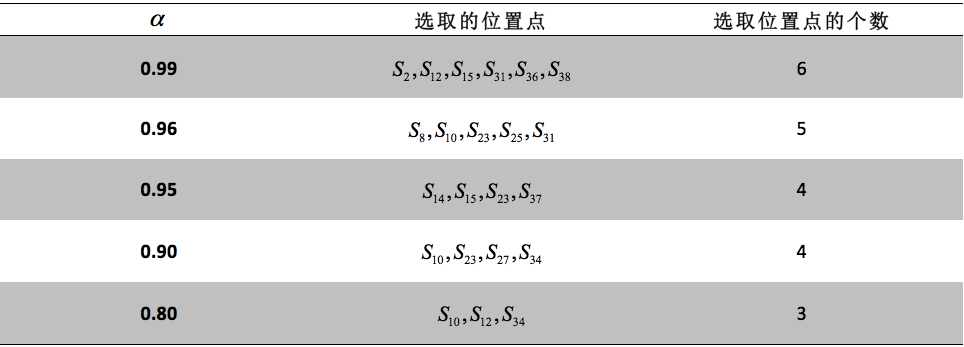
\includegraphics[width=\textwidth]{biaoge2.png}  
\end{figure}
\end{frame}
\begin{frame}
  在小规模的QoE测量网进行测试,备选位置点数为4,用户数为5
  \begin{figure}[htbp]
  \centering
  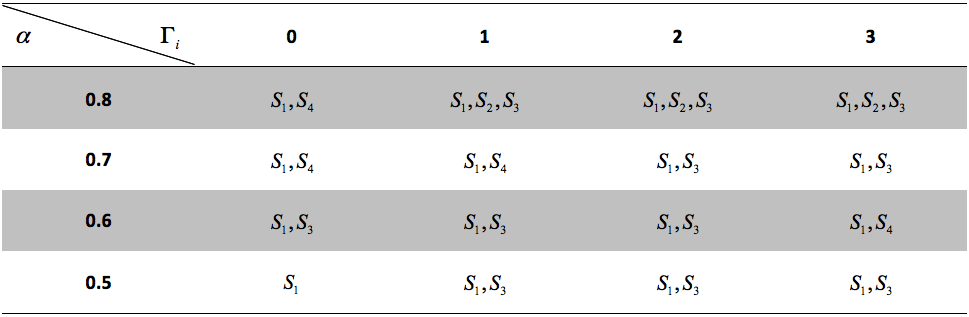
\includegraphics[width=\textwidth]{biaoge3.png}  
\end{figure}
\end{frame}
\section{后续进展}
\begin{frame}{后续进展}
考虑选取测量点时需要一定的费用,研究费用不确定的QoE测试网选址问题。
\begin{columns} 
\column{.5\textwidth} 
 \begin{align*}
\min \quad& \sum_{j\in J}c_jx_j \\
s.t. \quad& \sum_j a_{ij}x_j\geqslant 1, \quad \forall i\in I\\
& x_j \in \{0,1\},\quad \forall j\in J
\end{align*}
\column{.5\textwidth} 
\begin{align*}
\min &\quad \max_{F\in D}\mathbb{E}_{F}(\sum_{j\in E}c_jx_j) \\
s.t. \quad& \sum_j a_{ij}x_j\geqslant 1, \quad \forall i\in I\\
& x_j \in \{0,1\},\quad \forall j\in J
\end{align*}
\end{columns}


\end{frame}
% \begin{frame}
%   \begin{equation*}
%   \begin{cases}
%  P(c\in \varphi)=1 \\
% (\mathbb{E}(c)-\mu )^T \Sigma^{-1}(\mathbb{E}(c)-\mu )\leq \gamma_1,\\
% \mathbb{E}[(c-\mu )(c-\mu)^T] \preceq \gamma_2 \Sigma ,
% \end{cases}
% \end{equation*}
% \end{frame}
% \begin{frame}
%   \begin{align*}
% \min&\quad(\gamma_2\Sigma -\mu \mu^T)\cdot Q+r+\Sigma\cdot P-2\mu^Tp+\gamma_1s\\
% s.t. &\quad Q\succeq 0 \\
%  &\quad \begin{bmatrix} P&p\\p^T&s \end{bmatrix} \succeq 0\\
%  &\quad \begin{bmatrix} Q & p+Q\mu +\frac{x}{2} \\ (p+Q\mu +\frac{x}{2})^T &r \end{bmatrix} \succeq 0\\
% &\quad \sum_j a_{ij}x_j\geqslant 1, \quad \forall i\in I=\{1,2,\cdots,n\}\\
% & x_j \in \{0,1\},\quad \forall j\in J=\{1,2,\cdots,m\}
% \end{align*}
% 其中$A\cdot B=tr(AB),r$,$Q$,$\begin{bmatrix} P&p\\p^T&s \end{bmatrix}$是约束对应的拉格朗日乘子。
% \end{frame}
\begin{frame}
  
   整理成一篇系统的硕士学位论文。

完成撰写:2016.03

答辩时间:2016.05
\end{frame}
\section{论文情况}
\begin{frame}{论文情况}

 \begin{itemize}
   \item  {\em 服务网络QoE测试节点鲁棒选址问题研究},网络新媒体技术, 2015.11
   \item  {\em 考虑节点失效的QoE测量点鲁棒选址问题研究},在投
 \end{itemize}
  

\end{frame}



% \begin{frame}[t]{提出问题}
% 以视频为例:对于不同的用户来说,不同的视频网站服务效果是不一样的。当用户观看视频的时候,需要针对不同用户的不同业务类型为其推荐服务效果最好的视频网站,而直接要求用户自己来测试往往是不现实的。

% 所以我们需要{\color{blue}在服务网络中部署少量的一些点来模拟用户测试不同网站的服务效果。希望部署的点尽量少,同时又能比较准确的反映网络中所有用户获取不同服务的质量情况。}对于上述问题:
% \begin{itemize}
% 	\item  假设有一个可以部署测量点的备选位置点集,即可以在这些备选位置中选出一部分点来代表用户。
% 	\item 假设已经知道每个备选位置点可以代表哪些用户。
% \end{itemize}
% 那么,QoE 测量网选点问题要解决的是如何选择尽可能少的点来代表尽可能多的用户。
% \end{frame}

% \begin{frame}{问题抽象}
% 该问题可以抽象为图论中的集覆盖问题。

% 集覆盖问题是经典的NP-Hard类优化问题,对它的研究一部分集中在基于分支定界思想的完整算法,另一部分集中于启发式算法,如模拟退火算法,遗传算法,蚁群算法等。
% \begin{exampleblock}{实际情况}

% 实际情况中,各备选位置点可以代表的用户并不清楚,采用离散的情景描述不确定性,寻找一个鲁棒最优解,即{\color{red}选择尽可能少的点,使得在不同的情景下,这些点都可以覆盖全部的用户。}

% 考虑到实际选点问题中不确定因素的影响,我们将建立了QoE测量网选点问题的鲁棒选址集覆盖模型,进而以贪心算法为基础提出了一种求解鲁棒集覆盖问题的算法。
% \end{exampleblock}
% \end{frame}
% \section{选址模型}
% \begin{frame}{问题重述}
% $E=\{e_1,e_2\cdots,e_n\}$: QoE测量网用户集\\
% $e_i,i=1,2,\cdots,n$: 需要测量的网点\\
% $S=\{S_1,S_2,\cdots,S_m\}$: $E$的一族子集,为用来测试各网点使用不同网站服务效果的备选的测量位置点集\\
% $S_j,j=1,2,\cdots,m$: 备选测量位置点\\

% 假设测量网用户集$E$和备选的测量位置点集$S$均为{\color{red}有限}集。
% \begin{block}{QoE测量网点选址问题}
% 	从备选的测量位置点集$S$中选择合理的位置点,使QoE测量网用户集$E$中任意网点接受不同网站的服务时,至少有一个测量位置点可以测得其服务效果,同时使得选取的位置点个数最小。
% \end{block}


% \end{frame}

% \begin{frame}{简例}
% \begin{block}{抽象问题}
% 	给定元素的集合$E$,以及$E$的一些指定的子集组成的集合$S$,求$S$的子集$C$,使得$C$中所有集合的并等于$E$,同时要求集$C$中包含的子集个数最少。
% \end{block}

% $E=\{1,2,3,4,5\}$,$S=\{\{1,2\},\{3,4\},\{2,4,5\},\{4,5\}\}$

% 找到能满足条件的集合可以有$C=\{\{1,2\},\{3,4\},\{4,5\}\}$或者$C=\{\{1,2\},\{3,4\},\{2,4,5\}\}$
% \end{frame}

% \begin{frame}[fragile]{选址模型}
% 由于各位置点对不同网点测量情况有所不同,用0-1测量矩阵$A=(a_{ij})_{n\times m}$描述备选位置点对网点的测量情况:\\
% $a_{ij}=1$表示测量位置点$S_j$可以有效测量网点$e_i$获得服务的质量情况,即$e_i\in S_j$,\\
% $a_{ij}=0$表示备选位置点$S_j$不能有效测量网点$e_i$获得服务的质量情况,即$e_i\notin S_j$。


% \end{frame}
% \begin{frame}
% \begin{block}{QoE测试节点选址模型}
% 	QoE测试节点选址模型可用0-1整数规划确切地描述如下:
% \begin{align}
% \min \quad& \sum_{j\in J}x_j \\
% s.t. \quad& \sum_j a_{ij}x_j\geqslant 1, \quad \forall i\in I=\{1,2,\cdots,n\}\\
% & x_j \in \{0,1\},\quad \forall j\in J=\{1,2,\cdots,m\}
% \end{align}
% \end{block}
% $x_j$: 0-1决策变量,$x_j=0$表示集合$S_j$未被选中,$x_j=1$表示选取集合$S_j$\\
% $a_{ij}$表示集合$S_j$是否包含$e_i$,当$e_i\in S_j$时为1,否则为0;

% 公式(1)表示所求备选位置点个数最少;\\
% 公式(2)表示$E$中任意元素$e_i$至少被集合覆盖一次,即每个网点服务质量情况至少可以被一个位置点测量;\\
% 公式(3)为完整性约束。
% \end{frame}
% \begin{frame}{鲁棒选址模型}
% %如果已知各个备选位置点$S_j$可以测试网站服务效果的用户范围,即
% 测量矩阵$A$已知时,为传统集覆盖问题,该问题已被证明是NP完全问题,无法在多项式算法时间内求解。

% 实际中各备选位置点在测试用户接受网站的服务效果时,对于不同的网站可以测试的用户范围也是不同的,也就是说各备选位置点可以代表的用户即$S_j$是不确定的。

% 鲁棒优化方法: 用离散的情景描述测试不同网站的服务效果的不确定性,也就是用不同情景代表不同的网站。由于备选位置点测试不同网站时覆盖用户的范围不同,需要找到一个最优解使它对不确定参数观测值不敏感,即{\color{red}选择尽可能少的点,使得在不同的情景下这些点都可以覆盖全部的用户,并且所选的备选位置点能够测量各用户使用不同网站的服务效果}。
% \end{frame}





% 由于原问题是传统集覆盖问题,被证明在多项式算法时间内无法求解,鲁棒选址模型在原问题上考虑了离散情景使得问题的难度有所增加,考虑分析不确定因素的影响采用启发式算法进行求解。
% \end{frame}



% \section{模型求解}
% \begin{frame}{求解算法}
% 确定性选址问题属于集合覆盖问题,该问题无法在多项式算法时间内求解。目前求解效果好的是集覆盖的贪心算法
% \begin{block}{贪心算法(GSC)}
%   给定集覆盖问题的一个实例,从 $S$中选取一个覆盖$E$中元素最多的集合,然后把$S$所覆盖的元素从$E$中去除,重复以上操作直至覆盖$E$中所有元素。算法步骤如下:

%   步骤1. 输入$E$, $S=\{S_j|j\in J\}$, $X\leftarrow E$, $C=\varnothing$;

%   步骤2. 重复以下操作直至$X=\varnothing$: 选择$j$使得$S_j$覆盖的$X$元素数目最大,$C=C\cup \{j\}$, $X=X-S_j$.
% \end{block}
% \end{frame}

% \begin{frame}{启发式算法}
% 借鉴贪心算法,本文的算法思想是对备选位置点集中的集合进行处理,对任意两个集合都取并集得到新的集合,对新集合应用贪心算法的思想得到覆盖集,最后一步时对需要覆盖的元素进行判断: 是否可以使用更少的集合数可将其覆盖,也就是说是否只需一个集合就能得到所需的集合覆盖,并输出最终解。
% \begin{alertblock}{算法流程}
% 步骤1. 输入$E$, $S=\{S_j|j\in J\}$;

% 步骤2. $X\leftarrow E$, $C=\varnothing$, $\Delta = \{S_{ij}|S_{ij}=S_i\cup S_j, \forall i <j\in J\}$, $k=1$;

% 步骤3. 若$X\neq \varnothing$,判断$\Delta$是否为空,若为空集,$C=S$,输出C;否则$Y\leftarrow X$。选取$S_{ij}$使得其覆盖的$E$元素数目最大,记所得$S_i,S_j$为$u_k,v_k$;$X=X -S_{ij}$,$C=C\cup\{S_i,S_j\}$,将$\Delta$中下标里含$i$与$j$的元素删掉,重复步骤3;

% 步骤4. 若$X = \varnothing$判断是否$Y\subset S_j,\forall j\in J$,若存在这样的$S_j$,$C=C-\{u_{k-1}\}-\{v_{k-1}\}+\{S_j\}$否则$C=C$;

% 步骤5. 输出所得$C$.

% \end{alertblock}

% \end{frame}
% \begin{frame}{鲁棒选址问题的求解步骤}
% 根据实际情况,对于上节提出的模型,对于不同的网站(即随着情景的变化),考虑几种特殊情形:
% \begin{itemize}
%   \item  备选位置点集$S$的所有元素覆盖能力均{\color{red}增强},各备选位置点$S_i$覆盖用户范围也变广,可覆盖的用户在原有基础上增多,即${\color{red}S_i^t \subset S_i^{t+1}},\forall i\in I,t\in T$
%   \item 备选位置点集$S$的所有元素覆盖能力均{\color{red}减弱},各备选位置点$S_i$覆盖用户范围变窄,可覆盖的用户在原有基础上减少,即${\color{red}S_i^t \supset S_i^{t+1}},\forall i\in I,t\in T$
%   \item 备选位置点集$S$中元素{\color{red}部分}覆盖能力{\color{red}增强},而{\color{red}部分}覆盖能力{\color{red}减弱},对应的覆盖用户范围增广或变窄,可覆盖的用户数在原有基础上增多或减少;即{\color{red}对任意$i\in I_1,t\in T,S_i^t \subset S_i^{t+1}$,对任意$i\in I_2,t\in T,S_i^t \supset S_i^{t+1}$,$I_1$和$I_2$分别表示覆盖能力增强和减弱的点集下标,满足$I_1\cup I_2=I$}。
% \end{itemize}
% 在上述几种特殊情形下,求得尽可能少的备选位置点使其在不同情景下均可覆盖全部用户,能够测量各用户使用不同网站的服务效果。
% \end{frame}
% \begin{frame}
% 	对于鲁棒选址问题,我们可以分别求得不同情景下的覆盖集,再选出也可以在其他情景下覆盖全部用户的覆盖集,对所有情景下均可覆盖全部用户的覆盖集选取目标函数值最小也就是覆盖集合个数最少的方案。但由于每个情景下所有的覆盖集个数较多,当问题规模增大、情景增多时枚举将大大增加算法运行的时间。
% 本文考虑最坏的情景,也就是该情景下需要选取的最少备选点数较其他情景最多。
% \begin{itemize}
% 	\item  情形(1),情景$t=1$时,备选位置点集中元素覆盖能力最弱,鲁棒选址问题转化为情景$t^*=1$下的确定性集覆盖问题,只需求解备选位置点集为$S^{t^*}=S^1$的集合覆盖问题。
% 	\item 情形(2),容易得到最坏情景$t$取最大值$\max$时,情景$t=\max$下求得的覆盖点集在其他情景下也一定可以覆盖全部的用户,鲁棒选址问题转化为情景$t^*=\max$下的确定性集覆盖问题,我们只需要求解备选位置点集为$S^{t^*}=S^{\max}$的集合覆盖问题。
% 	\item 情形(3),我们构造新的情景$t^*$使得所有备选点集在该情景下覆盖的用户数最少。令$S^{t^*}=S^1_{I_1}\cup S_{I_2}^{\max}$得到新的情景,鲁棒选址问题转化为情景$t^*$下的确定性集覆盖问题。
% \end{itemize}

% \end{frame}

% \begin{frame}
% 对于鲁棒选址问题,我们可以分别求得不同情景下的覆盖集,再选出也可以在其他情景下覆盖全部用户的覆盖集,对所有情景下均可覆盖全部用户的覆盖集选取目标函数值最小也就是覆盖集合个数最少的方案。但由于每个情景下所有的覆盖集个数较多,当问题规模增大、情景增多时枚举将大大增加算法运行的时间。
% 本文考虑最坏的情景,也就是该情景下需要选取的最少备选点数较其他情景最多。
% \end{frame}


% % \begin{frame}
% %   \begin{figure}[htbp]
% %   \centering
% %   \includegraphics[width=\textwidth]{biao1.png}  
% % \end{figure}

% % \end{frame}


% \begin{frame}{总结}
% 用鲁棒选址集覆盖模型描述QoE测量网选点问题,并用基于贪婪算法给出的算法求得鲁棒解。仿真案例结果表明:鲁棒解适用于所有的情景,同时鲁棒解对应的目标值与各情景下确定性模型最优值相差不大,一定程度上降低了不确定性带来的风险,保证了所得备选点集在不同的情景下都能够覆盖全部的用户,进而测量各用户使用不同网站的服务效果,满足了不确定覆盖情景下QoE测量网选点问题的实际需求。

% 未来可以考虑将本文对备选位置点集不确定用其他方法描述进行求解,同时可将算法推广为对备选位置点集中个元素做并集运算。
% \end{frame}



\section{参考文献}\scriptsize
\begin{frame}[allowframebreaks]{参考文献}
[1] Jain R. Quality of experience [J]. IEEE Multimedia, 2004, 11(1): 96-97

[2] Jeffrey Spiess, Yves T’Joens, Raluca Dragnea, etc. Using Big Data to Improve Customer Experience and Business Performance [J]. Bell Labs Tech. J., 2014, 184.

[3] Roth.R. Computer solutions to minimum cover problems[J]. OR, 1969.

[4] Garey M R, Johnson D S. Computers and intractability: a guide to the theory of NP-completeness[M]. NewYork: WHFreeman,1979.


[5] Carlo Mannino, Antonio Sassano. Solving hard set covering problems [J]. Operations Research Letters,1995,181.

[6] J.E Beasley, P.C Chu. A genetic algorithm for the set covering problem [J]. European Journal of Operational Research,1996,942.

[7] Lessing L, DumitrescuI, Stützle T. A Comparison between ACO algorithms for the set covering problem[J]. Lecture Notes in Computer Science, 2004,3172:1-12

[8] Kouvelis P, Yu G. Robust discrete optimization and its applications[J]. Dordrecht: Kluwer Academic Publishers, 1997.

[9] Williamson D P. Lecture notes on approximation algorithms. IBM, 1998,3:12-19.

[10] Chvátal V. A greedy heuristic for the set covering problem[J]. Mathematics of Operations Research,1979,4:233-235.

[11] 红叶. 基于移动互联网业务的QoE建模与分析[D]. 北京邮电大学,2013.

[12] Drezner, z. Heuristic solution methods for two location problems with unreliable facilities. Journal of Operations Research Society,1987,38(6), 509-514.

[13] Snyder LV, Daskin MS. Reliability models for facility location: The expected failure cost case. Transportation Science ,2005,39:400-416.

[14] Berman O, Dmitry K, Menezes M. B. C, Facility Reliability Issues in Network p-median problem: Strategic Centralization and Co-Location Effects, Operations Research, 2007, 55(2): 332-350.

[15] Cui T, Ouyang Y F, Shen Z J M. Reliable facility location design under the risk of disruptions [J]. OR, 2010, 58(4): 998-1011.

[16] Peng P, Snyder L V, Lim A, et al. Reliable logistics networks design with facility disruptions [J]. Transportation Research Part B, 2011, 45(8): 1190-1211.

[17] Bertsimas D, Sim M. The price of robustness [J]. OR,2004,52(1).

[18] Dirk Degel, Pascal Lutter. A Robust Formulation of the Uncertain Set Covering Problem 2013.
%   \begin{thebibliography}{30}

%   \beamertemplatebookbibitems
%   % Start with overview books.

%  \bibitem{GJ} Garey M R, Johnson D S
%  \newblock{\em Computers and intractability: a guide to the theory of  NP-completeness.}
%  \newblock NewYork: WHFreeman,1979

% \bibitem{KY}Kouvelis P and Yu G
%  \newblock{\em Robust discrete optimization and its applications. } 
%  \newblock Dordrecht: Kluwer Academic Publishers, 1997.8-17

% % \bibitem{ } 
% % \newblock{\em  } 
% % \newblock  
% \beamertemplatearticlebibitems

% \bibitem{J}Jain R
% \newblock{\em Quality of experience}.
% \newblock IEEE Multimedia, 2004, 11(1): 96-97

% % \bibitem{R} Roth.R
% %  \newblock{\em  Computer solutions to minimum cover problems.} 
% %  \newblock  Operation Research, 1969, 17:455-465

%  \bibitem{MS} Carlo Mannino, Antonio Sassano
%  \newblock{\em Solving hard set covering problems } 
%  \newblock Operations Research Letters,1995,181

%  \bibitem{BC} J.E Beasley, P.C Chu
%  \newblock{\em A genetic algorithm for the set covering problem.} 
%  \newblock European Journal of Operational Research,1996,942

%  \bibitem{CV} Chvátal V
%  \newblock{\em  A greedy heuristic for the set covering problem.} 
%  \newblock Mathematics of Operations Research,1979,4:233-235.


%  \bibitem{ZZ} 张大陆, 祝嘉麒
%  \newblock{\em  网络传输中IPTV的QoE评估模型的研究.} 
%  \newblock  计算机工程与应用, 2013, 20: 71-76

%  \bibitem{W} 王文婧
%  \newblock{\em 移动云计算的QoE评价与优化研究 }
%  \newblock  北京: 北京邮电大学, 2013

%   \end{thebibliography}
\end{frame}

\begin{frame}

\begin{center}

  \Huge{谢谢!}
\end{center}

\end{frame}

\end{document}
